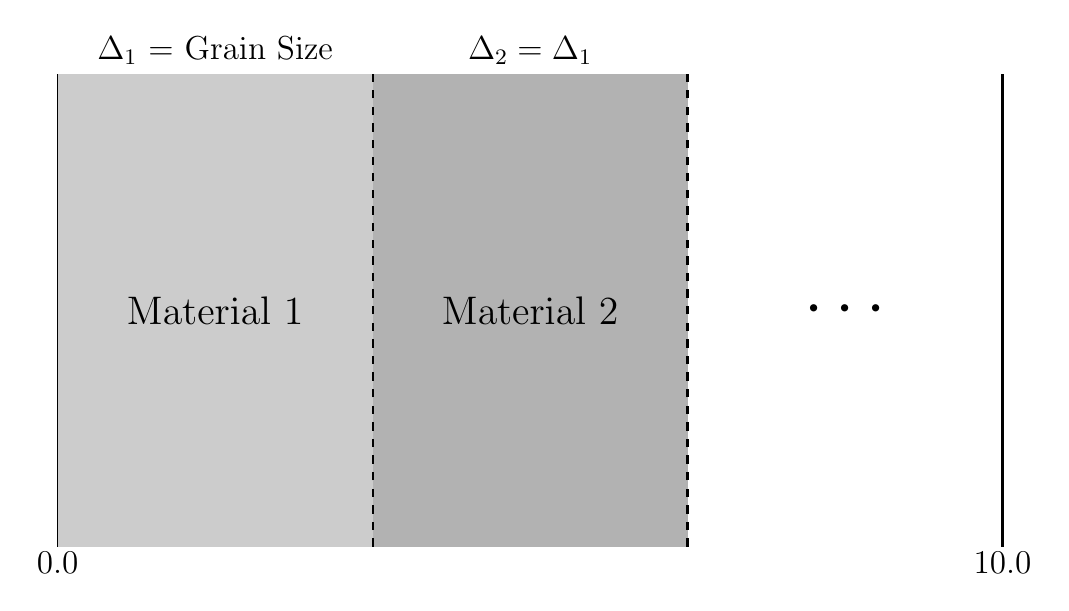
\begin{tikzpicture}
    \begin{scope}[thick,font=\scriptsize]

    \draw [-] (-3,-3) -- (-3,3) {};
    \draw [-] (9,-3) -- (9,3) {};
    
    \draw node at (-3,-3.2) {\large $0.0$};
    \draw node at (9,-3.2) {\large $10.0$};
    
    \fill[fill=black!20] (-3,-3) rectangle (1,3);
    \fill[fill=black!30] (1,-3) rectangle (5,3);
    
    \draw [dashed] (1,-3) -- (1,3) {};
    \draw [dashed] (5,-3) -- (5,3) {};
    
    \draw node at (-1,0) {\Large Material 1};
    \draw node at (3,0) {\Large Material 2};
    \draw node at (7,0) {\Huge{$\cdots$}};
    
    \draw node at (-1,3.3) {\large $\Delta_{1}$ = Grain Size}; 
    \draw node at (3,3.3) {\large $\Delta_{2} = \Delta_{1}$};

    \end{scope}
\end{tikzpicture}